%% Please fill in your name and collaboration statement here.
\newcommand{\studentName}{Kevin Zhang}
\newcommand{\collaborationStatement}{I collaborated on this assignment with Tomoya Hasegawa, Emily Wang, and Hugo Yen, got help from no one else, and referred to nothing else.}


%%%%%%%%%%%%%%%%%%%%%%%%%%%%%%%%%%%%%%%%%%%%%%%
\documentclass[solution, letterpaper]{cs121}
\usepackage{enumerate}
\usepackage{tikz}
\usepackage{pgf}
\usepackage{tikz}
\usetikzlibrary{arrows,automata}
\usepackage{hyperref}
\usetikzlibrary{automata,positioning}
\begin{document}
\header{0}{Due September 29, 2015 11:59pm}

%%%%%%%%%%%%%%%%%%%%%%%%%%%%%%%%%%%%%%%%%%%%%%%
\PART{Juan, Sam}
%%%%%%%%%%%%%%%%%%%%%%%%%%%%%%%%%%%%%%%%%%%%%%%
\problem{1+1+1+1+1+1+1}{3/4 page}

Determine the cardinality of each of the following sets (countably infinite, uncountably infinite, finite). If finite determine number of elements. Briefly justify each of your answers. You can assume $\Sigma = \{a, b\}$.

\subproblem $\{D: \text{ $D$ is a DFA that accepts the string } ab  \}$

\subproblem Set of all languages over the alphabet $\{ a\}$

\subproblem $\{P(\Sigma^*) \}$

\subproblem $\emptyset \times \mathbb{N}$

\subproblem Set of all syntactically correct OCaml programs. 

\subproblem $P(\Sigma^*)  \setminus  REG$ where $REG = \{L : L \text{ is a regular language} \}$ 

\subproblem $ REG  \setminus  P(\Sigma^*)$ 

\noindent\\$\textbf{Solution}$.

\noindent\\(A) $\textbf{Countably infinite}$; this set is the set of DFAs that recognize the set of languages $\{L \cup \{ab\} | L \in P(\Sigma^*)\}$.  Every DFA corresponds to a regular expression; hence, this set of DFAs is at most countably infinite, since the set of regular expressions is countably infinite as well.
\noindent\\\\(B) $\textbf{Uncountably infinite}$; the alphabet $\{a\}$ yields a set of strings defined by $\{a^*\}$ (which is countably infinite; simply map the length of each string to the corresponding natural number), and therefore the set of all languages over the given alphabet is a power set of a countably infinite set, resulting in an uncountably infinite set.
\noindent\\\\(C) $\textbf{Finite}$; this is just a set with one element in it.
\noindent\\\\(D) $\textbf{Finite}$; the cross product of the empty set with any other set yields the empty set.  Hence, the number of elements is 0.
\noindent\\\\(E) $\textbf{Countably infinite}$; note that any OCaml program is just a string, where the alphabet is the set of all characters used to write an OCaml program (which is obviously finite).  Hence, the set of valid OCaml programs is just a subset of the language given by $\{\Sigma^*\}$, where $\Sigma$ is the alphabet above.  But this language is a countably infinite set of strings (as all languages given by the Kleene star of a finite alphabet are).  The set of valid OCaml programs is also obviously not finite (consider an arbitrary amount of whitespace, for example); hence, it must be countably infinite.
\noindent\\\\(F) $\textbf{Uncountably infinite}$; we know that $P(\Sigma^*)$ is uncountably infinite (this is from lecture, and the proof is too long to go through here).  Moreover, the set of regular languages is countably finite (after all, every regular language is just a string constructed from the alphabet of characters used in writing a regular language).  We will prove later that subtracting a countably infinite set from an uncountably infinite set results in an uncountably infinite set; we use it here to prove that the given set is uncountably infinite.
\noindent\\\\(G) $\textbf{Finite}$; note that every regular language is in the power set of the set of strings given by $\Sigma^*$; hence, the given subtraction results in the empty set.  Hence, the number of elements is 0.

\problem {6}{1/4 a page}
Convert the following NFA into a DFA using subset construction. Provide a formal description (5-tuple) and diagram for full credit.


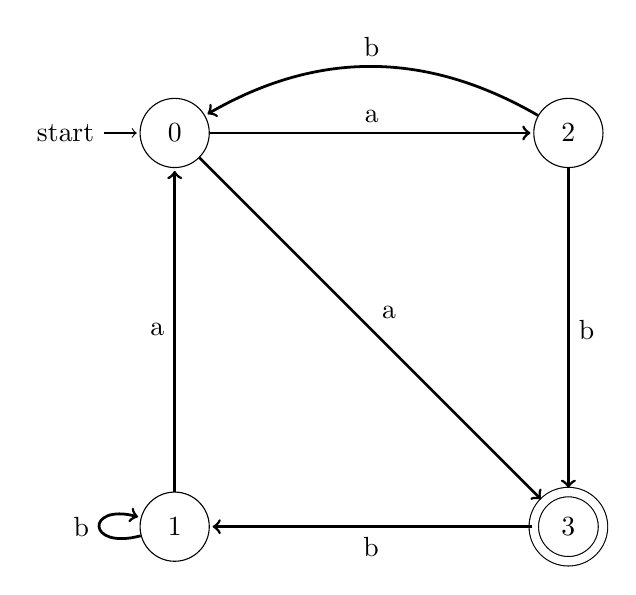
\begin{tikzpicture}[shorten >=1pt,node distance=3cm,on grid,auto] 
  \node[state, initial] (q_0) {$0$};
  \node[state] (q_1) [below=of q_0, yshift = - 2cm] {$1$};

  \node[state] (q_2) [right=of q_0, xshift = 2cm] {$2$};
  \node[state, accepting] [draw, double distance = 3pt] (q_3) [below=of q_2, yshift = - 2cm] {$3$};
  


  \path[->, line width=1pt]
    (q_0) 	edge node {a} (q_3)
	    edge node {a} (q_2)
    (q_1)		edge [loop left] node {b} ()
	    edge node {a} (q_0)			
    (q_2)		edge [bend right] node [swap] {b} (q_0)
	    edge node {b} (q_3)
    (q_3)		edge node {b} (q_1)
    
  ;

\end{tikzpicture}

\pagebreak
{\noindent} {\bf Solution.} 

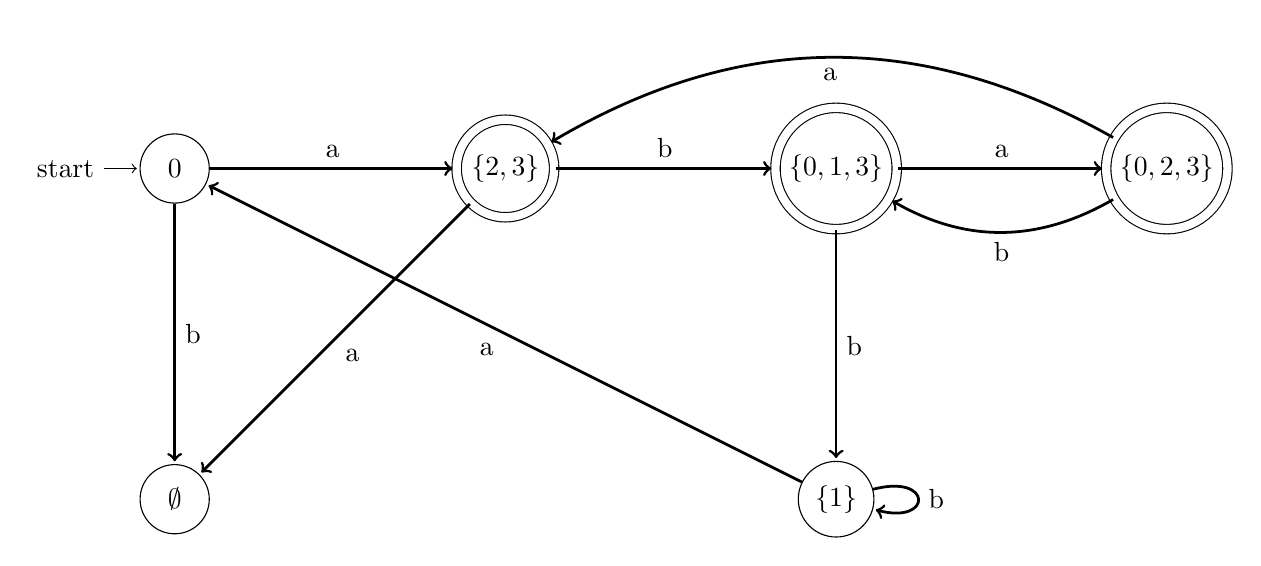
\begin{tikzpicture}[shorten >=1pt, node distance=3cm, on grid, auto]
	\node[state, initial] (q_0) {$0$};
	\node[state,accepting] [draw, double distance = 3pt] (q_1) [right=of q_0, xshift = 1.2cm] {$\{2,3\}$};
	\node[state,accepting] [draw, double distance = 3pt] (q_2) [right=of q_1, xshift = 1.2cm] {$\{0,1,3\}$};
	\node[state,accepting] [draw, double distance = 3pt] (q_3) [right=of q_2, xshift = 1.2cm] {$\{0,2,3\}$};
	\node[state] (q_4) [below=of q_2, yshift = -1.2cm] {$\{1\}$};
	\node[state] (err) [below=of q_0, yshift = -1.2cm] {$\emptyset$};
	
	\path[->, line width = 1pt]
		(q_0) 	edge 			node {a} (q_1)
		(q_0) 	edge				node {b} (err)
		(q_1) 	edge 			node {b} (q_2)
		(q_1) 	edge				node {a} (err)
		(q_2) 	edge 			node {b} (q_4)
		(q_2) 	edge 			node {a} (q_3)
		(q_3) 	edge [bend left] 	node {b} (q_2)
		(q_3) 	edge [bend right] 	node {a} (q_1)
		(q_4) 	edge [loop right] 	node {b} (q_4)
		(q_4) 	edge 			node {a} (q_0)
	;
\end{tikzpicture}

\noindent\\\\The above DFA = $(M', \Sigma', \delta', q_0', F')$ is defined as follows:
\begin{itemize}
	\setlength{\itemsep}{0pt}
	\item $M' = \{\{0\},\{2,3\},\{0,1,3\},\{0,2,3\},\{1\},\emptyset\}$
	\item $\Sigma' = \{a,b\}$
	\item $\delta' := $ 
	\begin{table}[h!]
		\begin{center}
			\begin{tabular}{ c | c | c }
				$q_0$ & a & b\\
				\hline
				$\{0\}$ & $\{2,3\}$ & $\emptyset$\\
				$\{2,3\}$ & $\emptyset$ & $\{0,1,3\}$\\
				$\{0,1,3\}$ & $\{0,2,3\}$ & $\{1\}$\\
				$\{0,2,3\}$ & $\{2,3\}$ & $\{0,1,3\}$\\
				$\{1\}$ & $\{0\}$ & $\{1\}$\\
			\end{tabular}
		\end{center}
	\end{table}
	\item $q_0' = \{0\}$
	\item $F = \{\{2,3\},\{0,1,3\},\{0,2,3\}\}$
\end{itemize}

\noindent The reject state and transitions to rejection are omitted.

\problem{3+2+3}{3/4 page}
\subproblem
Prove that if $A$ is an uncountable set and $B$ is a countable set, then 
$A \setminus B$ is uncountable.

\vspace{-4pt}
\subproblem
Find 2 examples: one where the intersection of two countably infinite sets
is finite and another where is countably infinite.

\vspace{-4pt}
\subproblem
Find 3 examples: one where the intersection of two uncountably infinite sets
is finite, another where it is countably infinite, and another where it is
uncountable.

\def\gsim{\mathrel{\rlap{\lower4pt\hbox{\hskip1pt$\sim$}}
    \raise1pt\hbox{$>$}}}                % greater than or approx. symbol
\def\notgsim{\mathrel{\rlap{\lower4pt\hbox{\hskip1pt$\sim$}}
    \raise1pt\hbox{$\not>$}}}                % greater than or approx. 
\def\notsim{\mathrel{\rlap{\hbox{$\sim$}}
    \hbox{$\not$}}}

\pagebreak
\noindent\\ {\bf Solution.}
\noindent\\\\ (A) Suppose that $A \setminus B$ is countable.  Then since the union of two countable sets is countable, $(A \setminus B) \cup B$ is countable.  But $(A \setminus B) \cup B$ is just $A$, which is uncountable; a contradiction!  Thus, $A \setminus B$ cannot be countable.
\noindent\\\\ (B) For the first example, let $A$ be the positive integers and $B$ be the positive integers.  Their intersection is the empty set, a finite set.  \\\indent For the second example, let $A$ be the positive integers and $B$ be the integers.  Their intersection is just $A$, which is countably infinite.
\noindent\\\\ (C) For the first example, let $A$ be the positive reals and $B$ be the negative reals.  Their intersection is the empty set, a finite set.  \\\indent For the second example, let $A$ be the positive reals and $B$ be the negative reals joined with the integers.  Their intersection is the positive integers, which is countably infinite.  \\\indent For the last example, let $A$ be the positive reals and $B$ be the reals.  Their intersection is the positive reals, which is uncountably infinite.
%%%%%%%%%%%%%%%%%%%%%%%%%%%%%%%%%%%%%%%%%%%%%%%
\PART{Cecilia and Charles}
%%%%%%%%%%%%%%%%%%%%%%%%%%%%%%%%%%%%%%%%%%%%%%%
	
\problem {each part 1}{1/2 page}
Translate the following languages over $\Sigma=\{a,b\}$ from English description to regular expressions, or vice versa.
\subproblem $L = \{w\in\Sigma^*:$ the second letter of $w$ is the same as the last letter, $|w| \geq 2 \}$
\subproblem $L = \{w\in\Sigma^*:$ every $a$ is followed by an odd number of $b$'s$\}$
\subproblem $(a(a\cup b)^*b) \cup (b(a\cup b)^*a)$
\subproblem $L = \{w\in\Sigma^*:w$ has at least two $b$'s and at most one $a\}$
\subproblem $L = \{ w \in \Sigma^* :  \text{every }b\text{ in }w\text{ has a }b\text{ directly before it} \}$ 
\subproblem $(b^* \cup ba)^*$ \\
	
\noindent {\bf Solution.}
\noindent\\\\(A) $\Sigma a(\Sigma^*)a \cup \Sigma b(\Sigma^*)b \cup \Sigma\Sigma$
\noindent\\(B) $b^*(ab(bb)^*)^*$
\noindent\\(C) $L = \{w \in \Sigma^*$ : start and end with different letters, $|w| \ge 2\}$
\noindent\\(D) $bb(b^*)a \cup b(b^*)ab(b^*) \cup abb(b^*) \cup bb(b^*)$
\noindent\\(E) $a^*$
\noindent\\(F) $L = \{w \in \Sigma^*$ : every $a$ has at least one $b$ before it$\}$
	
\pagebreak
\problem {9}{1 page}
Using the formal construction from the lecture notes or Sipser, convert the shown NFA to a regular expression. Please remove only one state per step. Show all steps or give explanation for steps not shown. 
	
Note: There is no need to add an additional final state and add epsilon transitions to that state. If you are texing your solutions, you can just copy paste the NFA from the problem statement below and modify it. You can also use http://madebyevan.com/fsm/.
	
\bigskip

\begin{tikzpicture}[->,>=stealth',shorten >=1pt,auto,node distance=6cm,semithick]
\tikzstyle{every state}=[fill=none,draw=black,text=black]

\node[initial,state] (0)                    {$q_0$};
\node[state]         (1) [right of=0] {$q_1$};
\node[state]         (2) [below right of=0] {$q_2$};
\node[accepting,state]         (3) [right of=1]       {$q_3$};

\path(0) edge              node {$a$} (1)
	edge               node {$b$} (2)
(1) edge   [bend right]    node {$b$} (2)
	edge        node {$b$} (3)
(2) edge 	[bend right]		node{$a$}(1)
	edge [loop below] node {$a$}(2)
(3) edge [loop below] node {$b$} (3)
	edge [loop right] node {$a$}(3)
;
\end{tikzpicture}
	
\pagebreak

\noindent {\bf Solution.}

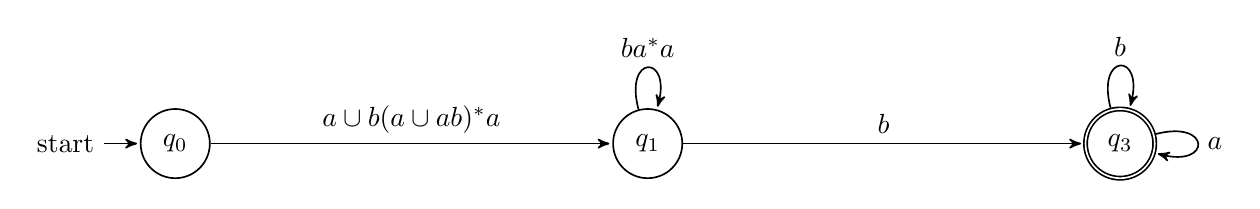
\begin{tikzpicture}[->, >= stealth', shorten >= 1pt, auto, node distance = 6cm, semithick]
\tikzstyle{every state}=[fill=none, draw=black, text=black]

\node[initial,state]		(0)			{$q_0$};
\node[state]			(1) [right of=0] 	{$q_1$};
\node[accepting,state]	(3) [right of=1] 	{$q_3$};

\path
	(0) 	edge 			node {$a \cup b(a \cup ab)^*a$} 	(1)
	(1) 	edge 			node {$b$} 					(3)
	(1)	edge [loop above]	node {$ba^*a$}					(1)
	(3) 	edge [loop above] 	node {$b$} 					(3)
		edge [loop right] 	node {$a$}					(3)
;

\end{tikzpicture}

\vspace{0.5cm}

\noindent We try to remove $q_2$ here; note that every path from $q_0$ to $q_1$ through $q_2$ starts with an $b$ and ends with an $a$, and intermediate steps from $q_2$ to itself are either $a$ or $ab$.  Thus, any route that goes from $q_0$ to $q_1$ through $q_2$ takes the form $b(a \cup ab)^*a$; join this with the other paths (just $a$) and we get all paths from $q_0$ to $q_1$.  Now, we also account for paths from $q_1$ to itself through $q_2$; these loops are of the form $ba^*a$.

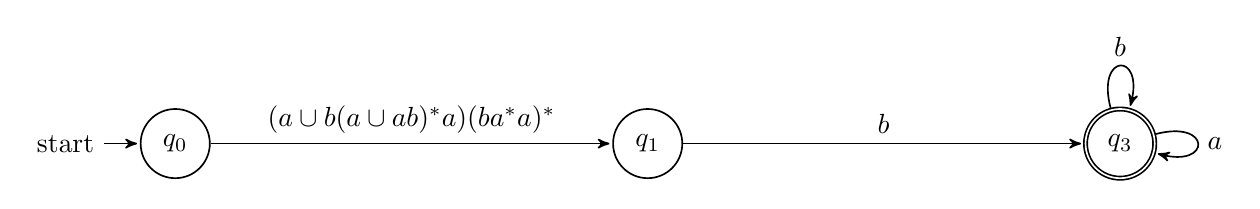
\begin{tikzpicture}[->, >= stealth', shorten >= 1pt, auto, node distance = 6cm, semithick]
\tikzstyle{every state}=[fill=none, draw=black, text=black]

\node[initial,state]		(0)			{$q_0$};
\node[state] 			(1) [right of=0] 	{$q_1$};
\node[accepting,state]	(3) [right of=1] 	{$q_3$};

\path
	(0) 	edge 			node {$(a \cup b(a \cup ab)^*a)(ba^*a)^*$} 	(1)
	(1) 	edge				node {$b$}								(3)
	(3) 	edge [loop above] 	node {$b$} 								(3)
		edge [loop right] 	node {$a$}								(3)
;

\end{tikzpicture}

\vspace{0.5cm}

\noindent Now we combine the loop into the left path.

\begin{tikzpicture}[->, >= stealth', shorten >= 1pt, auto, node distance = 6cm, semithick]
\tikzstyle{every state}=[fill=none, draw=black, text=black]

\node[initial,state]		(0)			{$q_0$};
\node[accepting,state]	(3) [right of=1] 	{$q_3$};

\path
	(0) 	edge 			node {$(a \cup b(a \cup ab)^*a)(ba^*a)^*b$} 	(3)
	(3) 	edge [loop above] 	node {$b$} 					(3)
		edge [loop right] 	node {$a$}					(3)
;

\end{tikzpicture}

\vspace{0.5cm}

\noindent Now remove $q_1$; just join $b$ with the previous path to create the path from the start to final state.

\vspace{0.5cm}

\begin{tikzpicture}[->, >= stealth', shorten >= 1pt, auto, node distance = 6cm, semithick]
\tikzstyle{every state}=[fill=none, draw=black, text=black]

\node[initial,state]		(0)			{$q_0$};
\node[accepting,state]	(3) [right of=1] 	{$q_3$};

\path
	(0) 	edge 			node {$(a \cup b(a \cup ab)^*a)(ba^*a)^*b(a \cup b)^*$} 	(3)
;

\end{tikzpicture}

\vspace{0.5cm}

\noindent The last step is easy; we just add an arbitrary string to the end of our expression to remove the self-loops from $q_3$.  The result is $(a \cup b(a \cup ab)^*a)(ba^*a)^*b(a \cup b)^*$.  This can be simplified as follows:

\begin{align}
(a \cup b(a \cup ab)^*a)(ba^*a)^*b(a \cup b)^* &= (a \cup (ba^*a)^*)(ba^*a)^*b(a \cup b)^*
\\	&= (a(ba^*a)^* \cup (ba^*a)^*)b(a \cup b)^*
\\	&= (a \cup \vareps)(ba^*a)^*b(a \cup b)^*
\end{align}

\end{document}